\subsection{访问者模式(Visitor)}

\subsubsection{访问者模式简介}

访问者模式是一种软件设计模式,它允许在不更改对象结构的情况下添加新的操作。它通过创建一个访问者类来实现这一目的,该访问者类包含用于处理对象结构中的各个元素的方法。

访问者模式的一个常见应用场景是处理对象结构,例如处理树形结构或链表。在这种情况下,访问者模式允许在不更改树形结构或链表的情况下添加新的操作,从而使得程序更加灵活。

例如,假设我们有一个用于表示二叉树的类,如下所示:

\begin{lstlisting}
class BinaryTree {
  constructor(value) {
    this.value = value;
    this.left = null;
    this.right = null;
  }
}
\end{lstlisting}

我们可以创建一个访问者类来处理这个二叉树,如下所示:

\begin{lstlisting}
class TreeVisitor {
  visit(node) {
    // 处理当前节点

    if (node.left) {
      this.visit(node.left);
    }

    if (node.right) {
      this.visit(node.right);
    }
  }
}
\end{lstlisting}

在这个例子中,访问者类的 visit 方法可以用于遍历二叉树的所有节点,并对它们进行处理。我们可以通过更改 visit 方法的实现来添加新的操作,而不需要更改二叉树的定义。

访问者模式具有以下优点:

\begin{enumerate}
\item 访问者模式允许在不更改对象结构的情况下添加新的操作,从而使得程序更加灵活。
\item 访问者模式将有关的操作和数据结构分离开来,从而更容易实现和维护。
\item 访问者模式可以让程序更加模块化,使得操作和数据结构之间的耦合度降低。
\end{enumerate}

\begin{enumerate}
\item 访问者模式可能会导致代码难以理解和维护,特别是当有大量的操作和数据结构时。
\item 访问者模式可能会导致类的数量增加,从而增加系统的复杂度。
\item 访问者模式可能会导致性能问题,因为它需要多次遍历对象结构来实现操作。
\end{enumerate}

\subsubsection{访问者模式在项目中的应用}

\begin{figure}[H]
  \centering
  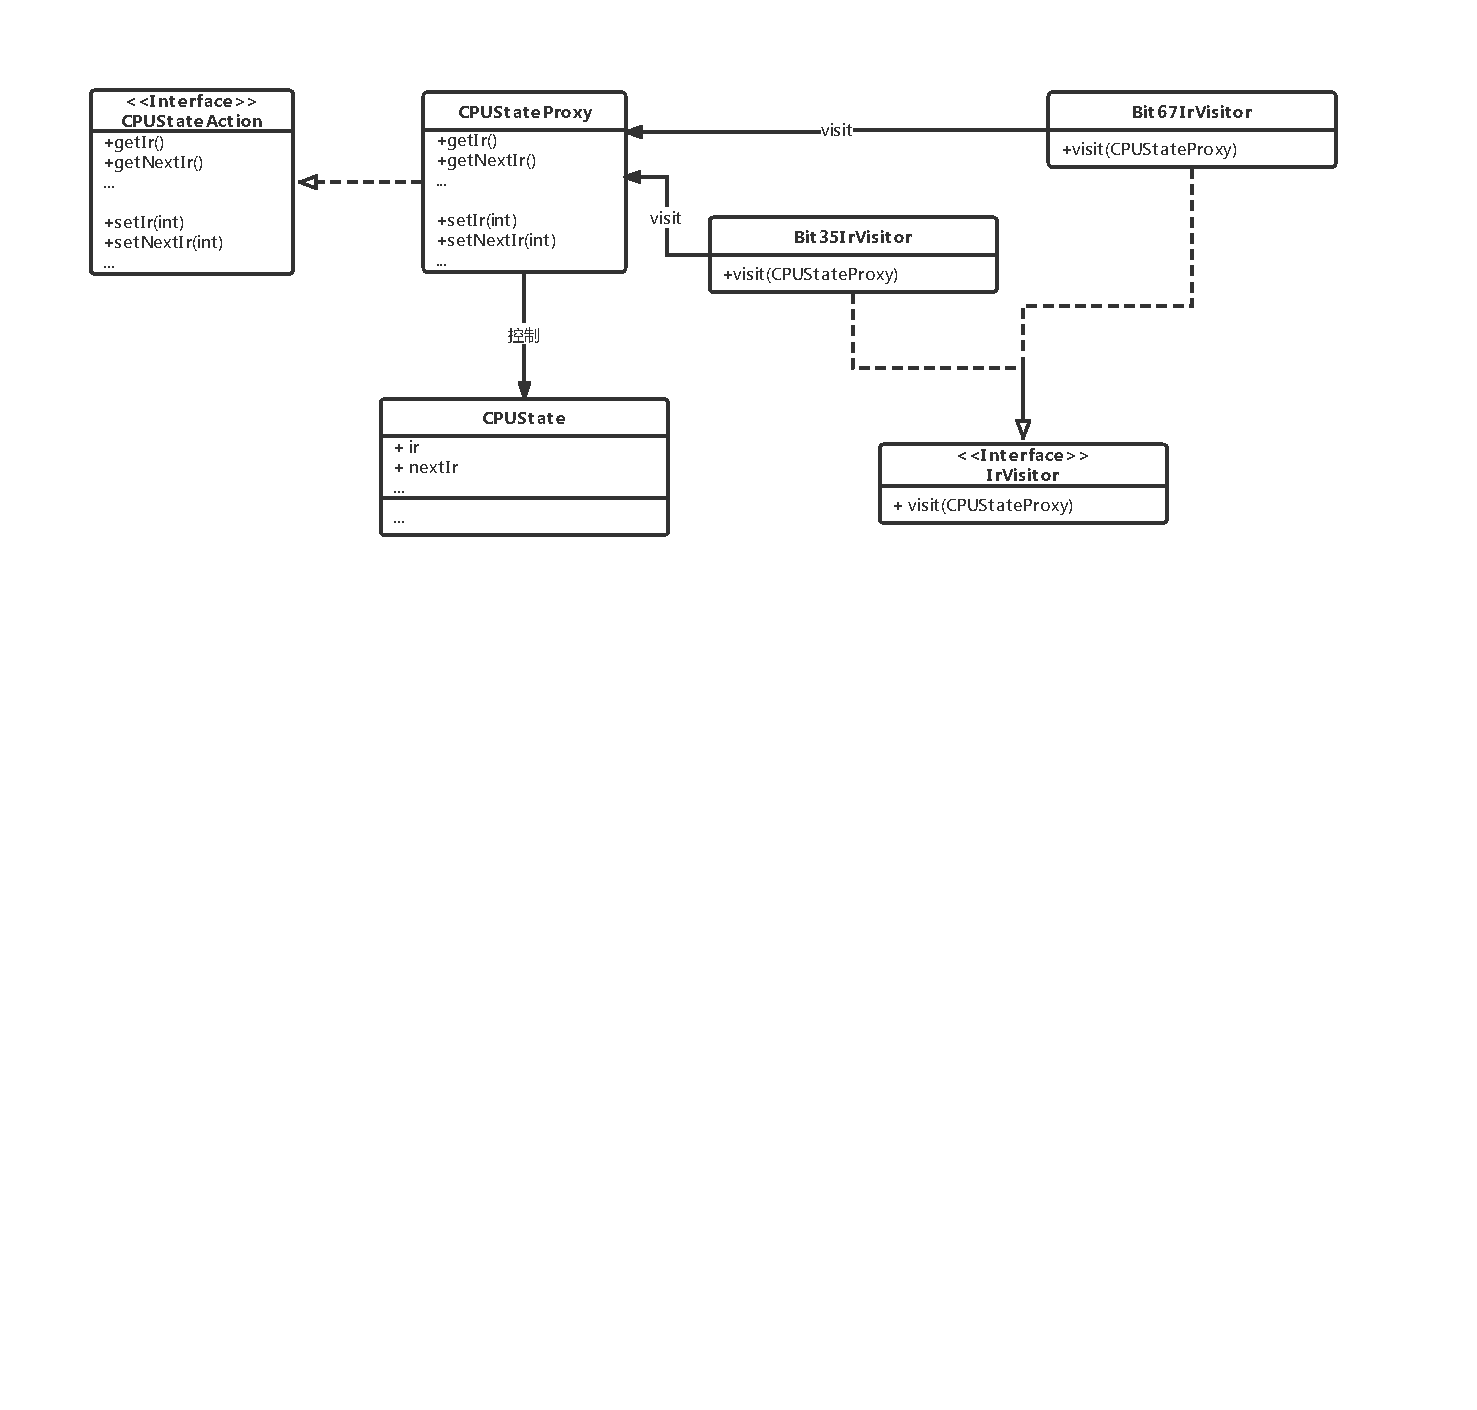
\includegraphics[width=0.9\textwidth]{figures/Visitor.pdf}
  \caption{访问者模式在 Slow6502 中的类图}
\end{figure}

在我们的项目中,CPU 对于 IR 寄存器的访问就是基于访问者模式实现的。CPU State 为一个 IR 中的每个元素提供多种访问方式,即 \lstinline{Bit67IrVisitor} 和 \lstinline{Bit35IrVisitor}。这样的设计可以允许在不更改 IR 寄存器结构的情况下添加新的操作,从而使得程序更加灵活。
